\documentclass[a4paper,10pt]{report}
%\usepackage[T1]{fontenc} % on some systems T1 looks ugly
%\usepackage[cyr]{aeguill}
\usepackage[utf8]{inputenc} 
\usepackage{ucs} 
\usepackage{times} 
\usepackage{graphicx} 
\usepackage{makeidx}
\makeindex
%\usepackage{german}
\usepackage{color}
\pagestyle{empty}
\defä{\"a} \defÄ{\"A} \defü{\"u} \defÜ{\"U} \defö{\"o} \defÖ{\"O} \defß{\ss}
\addtolength{\topmargin}{-.5in}        % repairing LaTeX's huge margins...
\addtolength{\textheight}{1in}        % more margin hacking
\addtolength{\textwidth}{1.5in}
\addtolength{\oddsidemargin}{-0.75in}
\addtolength{\evensidemargin}{-0.75in}
\newcommand{\myspec}[1]{\textbf{\textit{#1}}}
\newcommand{\mytt}[1]{{\tt #1}}


% \usepackage[pdftex]{graphicx}
% \DeclareGraphicsExtensions{.png,.pdf,.jpg,.jpeg}
% \usepackage[pdftex,
% bookmarks=true,
% bookmarksnumbered=true,
% pdfpagemode=None,
% pdfstartview=FitH,
% pdfpagelayout=SinglePage,
% colorlinks=true,
% urlcolor=magenta,
% pdfborder={0 0 0}
% ]{hyperref}

%%%%%%%%%%%%%%%%%%%%%%%%%%%%%%%%%%%%%%%%%%%%%%%%%%%
%interesting settings for the page layout

%\setlength{\hoffset}{-18pt}
%\setlength{\oddsidemargin}{0pt}  % left margin, odd pages
%\setlength{\evensidemargin}{9pt}  % left margin, even pages
%\setlength{\marginparwidth}{54pt} 
%\setlength{\textwidth}{481pt}  % set the text width to about 17cm
%\setlength{\marginparsep}{7pt}
%\setlength{\topmargin}{0pt}  % no margin on top
%\setlength{\headheight}{13pt}
%\setlength{\headsep}{10pt} 
%\setlength{\footskip}{27pt}
%\setlength{\textheight}{700pt}

%%%%%%%%%%%%%%%%%%%%%%%%%%%%%%%%%%%%%%%%%%%%%%%%%%%
%% miscalleneous packages

% \usepackage[frenchb]{babel} % use this if you are French
% \usepackage{verbatim} % include eg: source code easily
% \usepackage[utf8]{inputenc} or \usepackage[latin1]{inputenc}

% If you are on Fedora Core you may have problems with accents
% in this case replace the accentuated characters like this :
%
%  é -> \'e
%  è -> \`e
%  ê -> \^e and so on
%
% To automate the replacement you can make yourself a script
% here is a handy command-line for doing this :
% perl -pi -e "s/é/\\\'e/g" main.tex

\usepackage{amsmath}
% math extension - one probably wants to use symbols like '[' (written as '$[$')
% or $\epsilon$

% see mymacros.sty - print nice chapter headers
%\usepackage{mymacros}

%%%%%%%%%%%%%%%%%%%%%%%%%%%%%%%%%%%%%%%%%%%%%%%%%%%

% headers and footers for your document
%\usepackage{fancyheadings}
\usepackage{fancyhdr}

% count the number of pages for display on footer
\usepackage{lastpage}

% width of the line for headers and footers
%\headrulewidth 0.5pt
%\footrulewidth 0.5pt
%\addtolength{\headwidth}{\marginparsep}

% uncomment the following lines for headers
% the following command need picture files : "logo-school.jpg" 
% and "logo-company.jpg" in the project directory
%
%        \lhead{\sl \includegraphics[height=1.1cm]{logo-school}}
%        \chead{}
%        \rhead{\sl \includegraphics[height=1.2cm]{logo-company}}


\usepackage{ucs}
\usepackage[utf8]{inputenc}


%%%%%%%%%%%%%%%%%%%%%%%%%%%%%%%%%%%%%%%%
%document headers and footers
\lhead{}
\chead{}
\rhead{}
\lfoot{TU-Clausthal}
\cfoot{\thepage/\pageref{LastPage}}
\rfoot{ \today } % -> \rfoot{\number\month/\number\day/\number\year} 
\pagestyle{fancyplain}



\title{{\bfseries\Huge
\hrulefill\\
\hrulefill CP-PAW\hrulefill\\
\hrulefill Installation Guide\hrulefill\\
\hrulefill\\}
\hfill\\
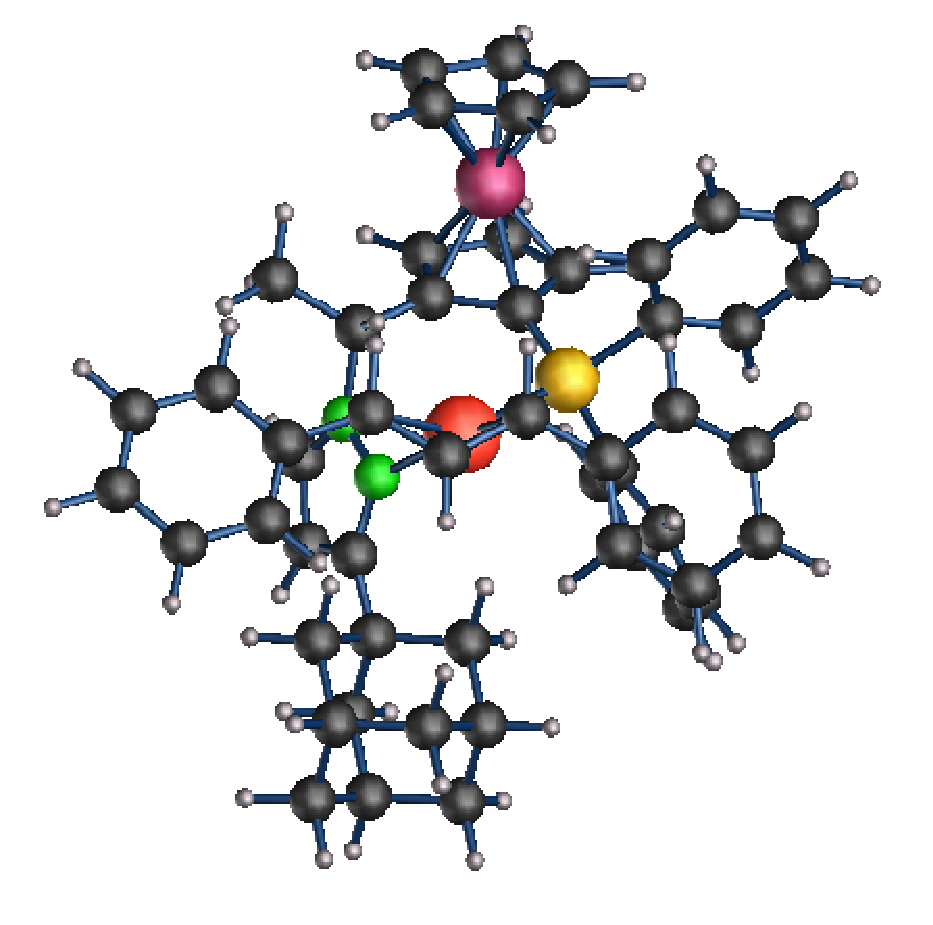
\includegraphics[width=9cm]{Figs/big.eps}
}
\date{\hrulefill\\Peter~E.~Bl\"ochl, Clausthal University of Technology\\(\today)}

\begin{document}
\maketitle
\tableofcontents

%======================================================
\chapter{Preface}
%======================================================
This installation guide goes back to a version of Clemens F\"orst, who
was the first to set up a rather comfortable installation procedure.
After Clemens left our group, I changed the installation procedure. In
this process I also undid some goodies that Clemens introduced,
because I was a complete newcomer to configure scripts.

After changing the installation in 2007, it was necessary to write a
new installation guide. The first step was taken by Axel Ehrich. Then
I took over.

As of now the Guide is still written partly in German. The translation
is still in progress.

I want to thank everybody, who contributed to the installation
procedure and this guide.

Peter Bl\"ochl

%======================================================
\chapter{Installation Guide}
%======================================================
%======================================================
\label{sec:vollstinst}
%=====================================================

%=====================================================
\section{Obtain the PAW distribution}
%=====================================================
The distribution of the CP-PAW code can be obtained from the CP-PAW
web page\index{CP-PAW web page}
\begin{center}
\mytt{https://orion.pt.tu-clausthal.de/paw}
\end{center}
following the link ``Download''. Access to the PAW distribution is
restricted to users with a valid license. You can apply for a license
on the same web-page. With a valid password you can obtain the codes.
You will also find so-called ``SETUP-files''\index{setup file}, which
were required by older PAW versions.

After you have given you Login name and Password you have reached the
``CP-PAW Download Page''. Following the link ``Sources'' on that page
you will find the actual distributions. We will denote it in the
following as \myspec{paw-distribution}\index{paw-distribution}. You
should always use the newest version. Even though it is called Beta,
it is currentlt our most safe version. The reason for naming it Beta
was to leav the option for a more stringent level.)

The \myspec{paw-distribution} is a gzipped tar file. You can see the
contents using the command
\begin{center} 
\mytt{tar tvfz} \myspec{paw-distribution}\mytt{.tgz}
\end{center}
The archive is expanded into the current directory exactly the way it
is listed here with the command
\begin{center}
\mytt{tar xvfz }\myspec{paw-distribution}\mytt{.tgz}
\end{center}
The directory created this way, whihc may be named ``paw-beta'' will
be denoted as \myspec{paw-directory}.


On other linux systems it may necessary to change the extension of the
file from \mytt{.tgz} to \mytt{.tar.gz}. Then one can unzip the file
with the command
\begin{center}
\mytt{gunzip } \myspec{paw-distribution}.tar.gz
\end{center}
The unzipped file is expanded with the command.
\begin{center}
\mytt{tar xvf } \myspec{paw-distribution}.tar
\end{center}

The directory \myspec{paw-directory} should look like this:
\begin{verbatim}
configure
configure.ac
dx
Makefile_bare.in
Makefile_targets.in
parameters
parms.example
parms.g95
README
src
\end{verbatim}

%=====================================================
\subsection{Download the Setup files}
%=====================================================
Once the PAW distribution has been obtained, download the so-called
setup files from the PAW Download page. This Tar file is similarly
expanded into a directory \myspec{paw-setupdir}. These data files will
be needed later to execute the CP-PAW code.

%=====================================================
\section{Installation of Compiler und Libraries}
%=====================================================
One needs
\begin{enumerate}
\item gnu-make (gmake; often simply make)
\item C-preprocessor (cpp)
\item a Fortran90 compiler, 
\item a numerical library for linear algebra, which corresponds to
BLAS\index{BLAS}. Examples are BLAS, ACML, MKL, ESSL.
\item a numerical library for linear algebra, which corresponds to
LAPACK\index{LAPACK}. Examples are LAPACK, ACML, MKL, ESSL.
\item a numerical library for Fast Fourier Transforms (FFT) such as
FFTW, ACML, MKL, ESSL.
\item An implementation of the Message Passing Interface
MPI\index{Mesasage Passing interface}\index{MPI}. Examples are MPICH
and MVAPICH.\index{MPICH}\index{MPICH}
\item depending on the, compiler a separate utility library is required.
\end{enumerate}
These items shall be installed. The reader should consult section
\ref{sec:software}, which contains additional information.

%=====================================================
\section{Adapt the parameter file}
%=====================================================
Now the distribution needs to be configured. The configuration
creates a set of make files, which are adapted to your system and
which take care of the final installation. More information about
configuring in general can be found in section
\ref{sec:configurebackground}.

The configure script\index{configure} needs a parameter file
``\myspec{parmfile}''\index{parameter file}\index{parmfile}, which
needs to be adapted. One should start with one of the examples listed
in the appendix \ref{sec:parmfiles}. The reader should then proceed to
section~\ref{sec:parmfile}, which contains a detailed description of
the parameters.

Note, that the format of the parameter file may not yet be final. Please
consult the current installation file.

%=====================================================
\section{Konfigurieren}
%=====================================================
Once the parameter file has been set up the configuration is done with the command
\begin{center}
\verb+./configure --with-parmfile=+\myspec{parmfile}
\end{center}
which is executed in the \myspec{paw-directory}. This process will
create a set of make files and a subdirectory tree 
\begin{center}
\myspec{paw-directory}\mytt{/bin/}\myspec{arch}
\end{center}
within \myspec{paw-directory}.  The name \myspec{arch} should be
unique and allows to maintain several installations simultaneously.

\begin{center}
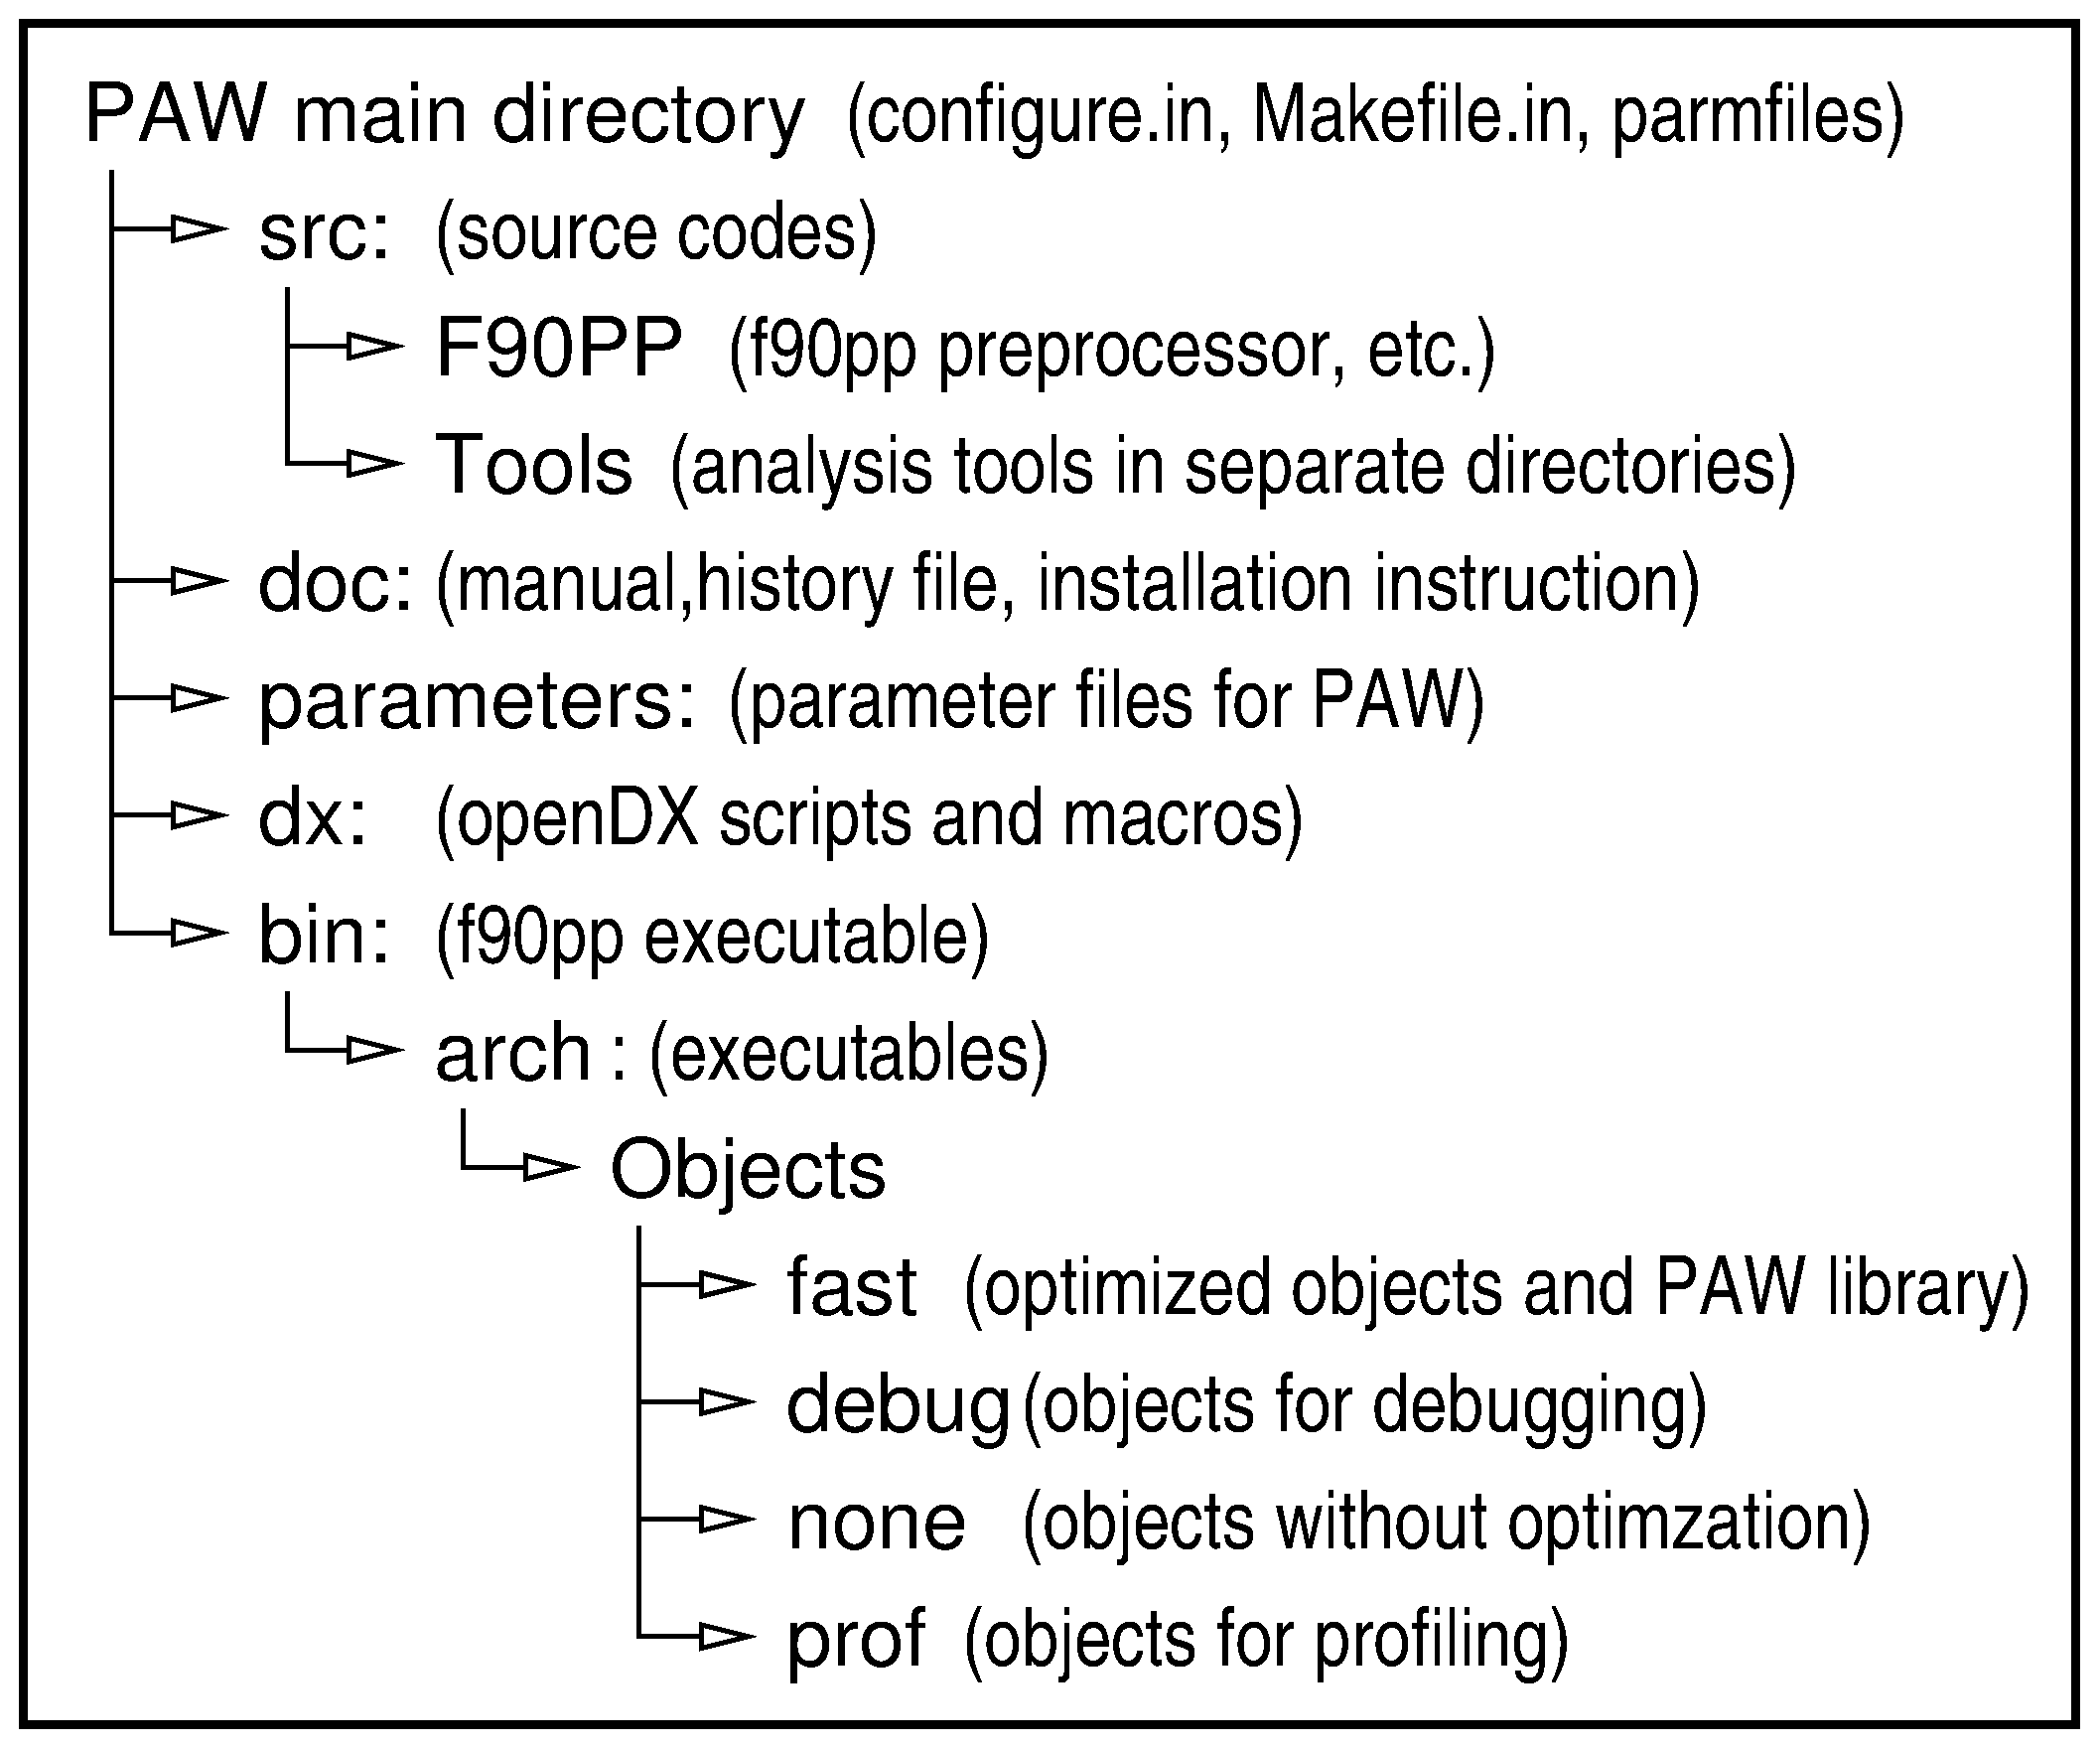
\includegraphics[width=0.6\linewidth]{Figs/PAWdirtree/pawdirtree.eps}
\end{center}

A successful configuration is indicated by a line
\begin{verbatim}
----done!---configuration completed successfully!--------------
\end{verbatim}
A typical printout of a configuration can be found in
appendix~\ref{sec:printoutconfigure}.


After each change in the \myspec{parmfile} execute \verb+./configure+.

%=====================================================
\section{Make}
%=====================================================
Next, one executes the command
\begin{center}
\mytt{make}
\end{center}
in the \myspec{paw-directory}. This compiles the sources and prepares
the executables.

In the beginning it may be wise to do the installation in small steps
so that Problems are observed early. The following sequence may be sensible
\begin{verbatim}
make docs
make none
make fast
make fast_parallel
make tools
make 
\end{verbatim}

The documentation is found in \myspec{paw-directory}\mytt{/doc}.  The
binaries are, for example,
\myspec{paw-directory}\mytt{/}\myspec{arch}\mytt{/paw\_fast.x}.

It is possible that optimization creates erroneous results. Therefore
the results of \mytt{/paw\_fast.x} should be compared once with
\mytt{/paw\_fast.x}. The latter does not contain optimization flags.

This completes the installation.



%======================================================
\chapter{Required software}
\label{sec:software}
%======================================================
\begin{itemize}
\item In section \ref{sec:compiler} we will provide information on the
installation of a FORTRAN compiler.
\item In section \ref{sec:libs} we will describe the installation of
numerical libraries and the Message Passing Interface.
\item  In section \ref{sec:utility} we will discuss the Utility library.
\end{itemize}

\noindent In addition to the above one will need
\begin{itemize}
\item a GNU C-preprocessor \mytt{cpp}
\item the GNU make tool. (Under the AIX operating system , the GNU
Make is named \mytt{gmake}. The default \mytt{make} of AIX will not
work with our make files.)
\end{itemize}

%======================================================
\section{FORTRAN Compiler}
\label{sec:compiler}
%======================================================
PAW is written in FORTRAN90. Later compiler versions such as FORTRAN95
and probably FORTRAN2003 can be used as well. 

In the following, we will mention some compilers that we have gained
experience with.
 
%====================================================
\subsection{G95}
\label{sec:g95}
%====================================================
\begin{itemize}
\item License: GPL (Open source)
\item Source: \textit{http://www.g95.org}
\item Problems: 
\begin{itemize}
\item The -std95 -std2003 compiler flags must be avoided, so that the
intrinsic function extensions can be used. In that case the g2c
library is not required. The g2c library is a fortran-to-C converter 
used for the interface of the support library calls. It is no more 
supported by GNU.
\item use the -fno-pic compiler flag under OS X.
\end{itemize}
\end{itemize}

%====================================================
\subsection{PGI Fortran Compiler}
%====================================================
\begin{itemize}
\item Suppplier: The Portland Group
\item Source: \textit{http://www.pgroup.com/}
\item Lizense: commercial
\item Problems: non known Problems
\item Remarks:
\begin{itemize}
\item The distribution of the PGI compiler already contains
precompiled librarues such as LAPACK, ACML, BLAS, MPICH.
\end{itemize}
\end{itemize}

%====================================================
\subsection{IFORT}
%====================================================
\begin{itemize}
\item Supplier: Intel
\item Source: Register on the 
page \textit{https://welcome.intel.com/Login.aspx}.
Then search for  ``Intel Fortran Compiler''.
\item License: commercial
\item Problems: 
\begin{itemize}
\item using the interprocedural optimization IPO the IFORT can produce
very large code. This caused the system to exceed the stack size. The
result was completely unpredictable behavior. If this is a problem
increase the stack size with \mytt{ulimit -s unlimited}. The stack
size can be controlled with \mytt{ulimit -a}.
\end{itemize}
\item Remarks:
\begin{itemize}
\item Very fast.
\end{itemize}
\end{itemize}


%====================================================
\subsection{XLF Compiler}
%====================================================
\begin{itemize}
\item Supplier: IBM
\item Source: \textit{http://www-306.ibm.com/software/awdtools/fortran/xlfortran/features/xlf-linux.html}
\item License: commercial
\item Remark: Only for the Power architecture of IBM
\item Problems: no known problems
\end{itemize}

%====================================================
\subsection{GFORTRAN}
%====================================================
\begin{itemize}
\item Supplier: Free Software Foundation
\item Source\textit{http://gcc.gnu.org/fortran/}
\item License: GPL (open source)
%\item Problems: We did not succed to compile PAW with gfortran.
\end{itemize}


%====================================================
\subsection{Absoft Fortran}
%====================================================
\begin{itemize}
\item Supplier: Absoft
\item http://www.absoft.com/
\item License: commercial
%\item Problems: We did not succed to compile PAW with an older version of 
%the Absoft compiler.
\end{itemize}


%====================================================
\section{Utility Library}
\label{sec:utility}
%====================================================
There are a few routines that are not part of teh fortran standard but
which are supplied by all compilers in similar form as
library. Sometimes they are treated like instrinsic functions as
Fortran extensions without the need to link a library.

The Utility Bibliothek is named differently by different
suppliers. IBM calls it ``Service and Utility Library'', Intel calls
it ``Portability Routines''. Traditional it is called Utility Library
U77, where 77 is related to the Fortran77 Standard.

Even though the library calls are nearly identical, they differ in the
kind parameter of the arguments. In order to avoid the corresponding
problems the CP-PAW code contains interfaces to the utility library
for the individual compilers. The specific interfaces are selected via
the C-preprocessor, if the corresponding parameters have been set in
as variable CPPFLAGS the parameter file (see Section~\ref{sec:cppflags}).

Consult the user guide of the corresponding compiler to find out if
If a utility library needs to be linked.

%====================================================
\newpage
\section{Numerical Libraries}
\label{sec:libs}
%====================================================

CP-PAW depends on numerical libraries for the following three
purposes. Often they are combined in asingle library.
\begin{itemize}
\item Basic Linear Algebra Subroutines (BLAS)\index{BLAS}:
mathematical library for elementary vector-matrix operations such as
vector and matrix multiplications.
\item Lineare Algebra PACKage (LAPACK)\index{LAPACK}: more complex
matrix operations such as eigenvalue solvers. (LAPACK relies on BLAS)
\item Fast Fourier Transformation Library (FFT):
As the name says: Fast Fourier transformations
\end{itemize}
These libraries are to a large part responsible for the efficiency of
the CP-PAW calculations.

There are standardized packages for the linear algebra routines,
namely the Linear Algebra PACKage (LAPACK) and the Basic Linear
Algebra Subprograms (BLAS) . The documentation for the LAPACK-Routines
can be found at
\begin{verbatim}
http://www.netlib.org/lapack/ 
\end{verbatim}
and the ones for BLAS at
\begin{verbatim}
http://www.netlib.org/blas/
\end{verbatim}
These two are a kind of standard for many other packages.

These packages are contained in libraries
such as
\begin{itemize}
\item IBM Engineering and Scientific Software Library (ESSL)
\item AMD Core Math Library (ACML)
\item Intel Math Kernel Library (MKL)
\end{itemize}

It is adviseable, not to use the libraries supplied by the operating system, but to complile them 
on the hardware, on which one intends to use them. These binaries are usually faster.

We found it useful to place all these libraries, that we created for
the current hardware into a directory \mytt{/home/tools} on the
specific computer. The advantage is that it facilitates installation
on parallel computer clusters, where the libraries are kept only on the
frontend.


The following table lists the combination of libraries that have been
tested.
\begin{center}
\begin{tabular}{|l|l|l|}
\hline
LAPACK& BLAS & FFT\\
\hline
LAPACK & ATLAS & FFTW2\\
ACML & ACML & FFTW2\\
ACML & ACML & ACML\\
MKL & MKL & FFTW2(MKL)\\
MKL & MKL & FFTW2\\
ESSL & ESSL & ESSL\\
\hline
\end{tabular}
\end{center}




%====================================================
\subsection{ATLAS-BLAS}
%====================================================
\begin{itemize}
\item Supplier: Open Source
\item Name: ATLAS=Automatically Tuned Linear Algebra Software
\item License: Open Source
\item Source \textit{http://math-atlas.sourceforge.net/}
\item Functions: BLAS
\item Installation:
\begin{itemize}
\item 
After unpacking the ATLAS distribution type make and follow the
instructions. Always use the default value ([y] or [n] by just typing
ENTER) until you arrive at
\begin{verbatim}
use express setup? [y]:
\end{verbatim}
Enter \texttt{no} and proceed taking the defaults if you like so.  Use
\texttt{f90} as \textsc{Fortran77} compiler (just needed to compile
the wrappers). As \texttt{F77 FLAGS} use
\begin{verbatim}
-YEXT_NAMES=LCS -YEXT_SFX=_ -O
\end{verbatim}
to ensure, that the linking works out.

Again take the default values until you reach the 
\begin{verbatim}
Enter C Flags (CCFLAGS) [-fomit-frame-pointer -O3 -funroll-all-loops]: 
\end{verbatim}
prompt.  Just use \texttt{-fomit-frame-pointer -O} and proceed accepting the defaults.

If you have compiled an ATLAS BLAS for different architectures (e.g. Pentium
and ATHLON), the corresponding libraries will be in different subdirectories of
the ATLAS distribution. You find these subdirectories in \texttt{ATLAS/lib}.
If there is just one, the configure script will chose it
automatically. 
\end{itemize}
\end{itemize}

%====================================================
\subsection{LAPACK}
%====================================================
\begin{itemize}
\item Name: LAPACK=Linear Algebra PACKage
\item Source: http://www.netlib.org/lapack/
\item Functions: LAPACK (The lapack package also contains slow BLAS
  routines. As the computational efficiency heavily depends on the
  performance of the BLAS library, one should always link a
  machine-optimized BLAS library.)
\item License: Open source
\item Installation:
\begin{enumerate}
\item Download \textit{lapack-lite-3.1.1.tgz} von
http://www.netlib.org/lapack/index.html
\item gunzip and untar the file
\item Copy and edit the file LAPACK/make.inc.example to LAPACK/make.inc.
\item Edit the file LAPACK/Makefile (see
http://www.netlib.org/lapack/lawn81/node13.html)
\item type make
\end{enumerate}
\end{itemize}

%====================================================
\subsection{FFTW}
\label{sec:FFTWinstall}
%====================================================
\begin{itemize}
\item Supplier: Massachusetts Institute of Technology (MIT)
\item Name: FFTW=Fastest Fourier Transform in the West
\item Source: \mytt{http://www.fftw.org/download.html}
\item License: open source
\item Remark
\begin{itemize}
\item The versions FFTW2 und FFTW3 are not compatible. 
Currently, the CP-PAW code only works with FFTW2.
\end{itemize}
\item Installation: 
\begin{enumerate}
\item download FFTW 2.1.5 from \mytt{http://www.fftw.org/download.html}.
\item Archiv mit \mytt{tar -xvzf Dateiname} entpacken
 \item Den Befehl \mytt{./configure --enable-i386-hacks} ausf\"uhren.
 The option \mytt{--enable-i386-hacks} takes advantage of the
 gcc/x86-specific performance hacks. (For the core2duo the option
 \mytt{--enable-i386-hacks} must be left out!)
\item On 32-bit architectures, change the following 
line in the file \textit{fftw/config.h} (At the end of the file):\\
\begin{verbatim}
 \#define F77_FUNC_(name,NAME) name ## __
\end{verbatim}
 Remove the last underscore so that the line reads as
\begin{verbatim}
  \#define F77_FUNC_(name,NAME) name ## _ 
\end{verbatim}
 \item  execute the command \textit{make}
\end{enumerate}
\end{itemize}


%====================================================
\subsection{ACML}
\label{sec:acml}
%====================================================
\begin{itemize}
\item Name: ACML=AMD Core Math Library
\item Supplier: AMD
\item Source: \mytt{http://developer.amd.com/acml.jsp}
\item Contains: FFT, LAPACK, BLAS
\item License: royalty-free license 
\item Installation: Untar the archive after downloading and follow
the installation instructions. 
\item Remarks: Available for Windows and Linux operating systems, and
  for the fortran compilers gfortran, ifort, pgi, pathscale, and nag.
\item Special instructions to use the ACML-internal FFT library:
\begin{itemize} 
\item use \verb+-DCPPVAR_FFT_ACML+ in the variable CPPFLAGS of the 
\myspec{parmfile} (see section~\ref{sec:cppflags}).
\item set the variable \verb+FFT_HEADER+ in the parameter file to 
the file gnu64/include/acml.h inside the acml directory.
\item do not include other FFT, LAPACK or BLAS libraries together 
with ACML.
\end{itemize}
\end{itemize}



%====================================================
\subsection{MKL}
%====================================================
\begin{itemize}
\item Supplier: Intel
\item Name: MKL=Math Kernel Library\index{MKL}
\item Source: \mytt{http://www.intel.com/cd/software/products/asmo-na/eng/307757.htm}
\item License: commercial (For Linux: free license for non-commercial entities)
\item Remarks: as of writing this the MKL 10.x does not yet work with CP-PAW.
\item Link the following libraries for MKL: mkl\_lapack, guide,
  pthread.  For i386 architecture also link mkl\_ia32 and for EM64T or
  AMD64 architectures link mkl\_em64t.œ
\item Installation:
\begin{enumerate}
\item Register at \mytt{https://welcome.intel.com/Login.aspx}
\item http://www.intel.com/cd/software/products/asmo-na/eng/307757.htm
\end{enumerate}
\item When using the MKL, the library ``pthread'' must be linked. (See
also appendix~\ref{sec:problempthread})
\end{itemize}


%====================================================
\subsubsection{FFTW der MKL}
%====================================================
The MKL contains an interface for FFTW calls and also supplies the
Routines for Fourier transforms.

In order to be able to use the FFTW of the MKL, one executes the
command \textit{make} from within the subdirectory
\textit{interfaces/fftw2xf} of the MKL directory This step requires
the intel fortran compiler and the intel C compiler.  The make command
constructs the library \textit{libfftw2xf\_intel.a} in the
corresponding directory \textit{mkl-libs}. In order to use this
library the paw-parameter file must be adapted. First one has to
adjust the value of \mytt{FFTDIR}.  Then one has to replace the value
\textit{fftw} by \textit{fftw2xf\_intel} in the variables
\textit{LIBS\_SCALAR } and \textit{LIBS\_PARALLEL}.

%====================================================
\subsection{ESSL}
%====================================================
\begin{itemize}
\item Name: Engineering and Scientific Subroutine Library (ESSL)
\item Supplier: IBM
\item Source: \mytt{http://www-03.ibm.com/systems/p/software/essl/index.html}
\item License: commercial
\item Remarks: 
\begin{itemize}
\item Only for IBM Hardware. Only for the AIX operating
system and for  Linux with Power architecture.
\item ESSL does not use the same calling sequences as LAPACK and
BLAS. However, PAW has a special interface for ESSL.
\end{itemize}
\item Covers: FFT, LAPACK, BLAS
\end{itemize}

%====================================================
\newpage
\section{Message Passing Interface}
%====================================================
The MPI (Message Passing Interface) is a protocoll, that allows a
distributed/parallel computing. The MPI must be compiled such that its
calls work with a single underscore.

Most hardware suppliers offer their own MPI implementations. 
There are also freely available MPI implementations, such as  MPICH and Open
MPI\textit{http://www.open-mpi.org/}. Our experiences are limited to
 MPICH,  MVAPICH, and the MPI of IBM.

%====================================================
\subsection{MPICH}
\label{sec:mpich}
%====================================================
MPICH is a free implementation of the MPI for  ethernet networks.

\begin{itemize}
\item Supplier: Argonne National Laboratory and Missisippi State University
\item Source http://www-unix.mcs.anl.gov/mpi/mpich1/
\item License: open source
\item Remarks:
\begin{itemize}
\item There is a new implementation of MPICH called MPICH2. According
to the supplier this is the currently recommendent implementation.
MPICH2 can be downloaded from\\
\centerline{\textit{http://www-unix.mcs.anl.gov/mpi/mpich2/index.htm}.}
It has not been tested with CP-PAW.
\end{itemize}
\item Installation:
\begin{enumerate}
\item Download of the most recent version from
\begin{center}
\textit{http://www-unix.mcs.anl.gov/mpi/mpich1/}
\end{center}
\item After unpacking, one can compile the MPI for PAW using the 
following script.

For G95
\begin{verbatim}
#!/bin/sh
export F90=g95
export F90FLAGS=-fno-second-underscore
export FC=g95
export FFLAGS=-fno-second-underscore
export FLINKER=g95
export RSHCOMMAND=ssh
./configure --enable-f77
\end{verbatim}
For Pathscale
\begin{verbatim}
#!/bin/sh
export CC=pathcc
export FC=pathf90 
export F90=pathf90 
export F90FLAGS=-fno-second-underscore 
export FFLAGS=-fno-second-underscore
export FLINKER=pathf90
export RSHCOMMAND=ssh
./configure -c++=pathcc -opt=-O3 --enable-f90 --enable-f90modules \
            --with-romio --disable-weak-symbols 
\end{verbatim}

\item execute \textit{make}.
\end{enumerate}
\end{itemize}

%====================================================
\subsection{MVAPICH}
\label{sec:mvapich}
%====================================================
MPICH is a free implementation of the MPI for  Infiniband networks.
\begin{itemize}
\item Supplier: Ohio State University
\item Source: \textit{http://mvapich.cse.ohio-state.edu/}
\item License: Open Source
\end{itemize}


%====================================================
\chapter{The Parameter File}
\label{sec:parmfile}
%====================================================

The parameter file is needed for the configuration of the compilation
process of CP-PAW. The parameter file selects the compiler, its
options, the numerical libraries, etc. 

An example is given in the following
section~\ref{sec:parms.example} and discussed later.

%============================================================================
\section{Example for a Parameter File}
\label{sec:parms.example}
%============================================================================
\begin{verbatim}
################################################################################
##_______________________architecture (arbitrary name)________________________##
ARCH="g95_guam"
##______________________flag for uppercase or lower case module file names____##
TUPPERCASEMOD="F"
##______________________flag for parallelization______________________________##
TPARALLEL="T"
##_______special rules for the configure script and f90 preprocessor__________##
SPECIAL="none"
##__________________DIRECTORIES containing LIBRARIES__________________________##
BLASDIR=""
LAPACKDIR="/home/tools/libs/acml3.0.0_64/gnu64/lib/"
FFTDIR="/home/tools/libs/fftw-2.1.5_no-second-underscore/"
MPIDIR="/home/tools/libs/mpich-1.2.6/"
##________________________ include file for fftw______________________________##
FFT_HEADER="${FFTDIR}/fortran/fftw_f77.i"
##_________________________________ include file for mpi "mpif.f90"___________##
MPI_HEADER="${MPIDIR}/include/mpif.h"
##_______F90 compiler and linker for scalar executables_______________________##
COMPILER_SCALAR="g95 -fno-second-underscore "
##_______F90 compiler and linker for parallel executables_____________________##
COMPILER_PARALLEL="g95 -fno-second-underscore "
##__________________standard compiler flags___________________________________##
FCFLAGS_NONE="-c "
#_______________________compiler flags for optimization_______________________##
FCFLAGS_OPT="-c -O3 -fshort-circuit -funroll-loops -fomit-frame-pointer -msse2"
##_______________________compiler flags for  profiling________________________##
FCFLAGS_PROF="-c -pg -O3 -fshort-circuit -funroll-loops  -msse2"
#_______________________compiler flags for debugging__________________________##
FCFLAGS_DBG="-c -g -std=f95 -Wall -ftrace=full  -fimplicit-none -fbounds-check"
#_______________________flags for linking_____________________________________##
LDFLAGS_SCALAR="-Wl,-dy -I${OBJDIR} -L${OBJDIR} -L${LAPACKDIR}  \
                 -L${FFTDIR}/fftw/.libs/"
#_______________________flags for linking_____________________________________##
LDFLAGS_PARALLEL="-Wl,-dy -I${OBJDIR} -L${OBJDIR} -L${LAPACKDIR} \
                  -L${FFTDIR}/fftw/.libs/ -L${MPIDIR}/mpe/lib"
#________________________external libraries (sequential)______________________##
LIBS_SCALAR="-Wl,-dn -lfftw -Wl,-dn -lacml -Wl,-dy -lg2c"
#___________________external libraries (parallel)_____________________________## 
LIBS_PARALLEL="-Wl,-dn -lfftw -Wl,-dn -lacml -Wl,-dy -lg2c -Wl,-dy -lmpe \
               -Wl,-dy -llmpe"
#________________________preprocessor variables_______________________________## 
CPPFLAGS="-DCPPVAR_COMPILER_G95 -DCPPVAR_FFT_FFTW \
          -DCPPVAR_LAPACK_LAPACK -DCPPVAR_BLAS_BLAS"
#________________________file extension_______________________________________## 
FEXT="f90"
################################################################################
\end{verbatim}
%$

%============================================================================
\section{Explanation of the Variables in the  Parameter File}
%============================================================================
\subsection{\mytt{ARCH}}
%
The value is a directory name, which will be created as
\begin{center}
\myspec{paw-directory}\mytt{/bin/}\myspec{arch}
\end{center}
This directory will contain all executables. It will also contain
subdirectories with the object files, module files,etc.

\subsection{\mytt{TUPPERCASEMOD}}

Different compilers name the module files either with uppercase
letters or lowercase letters. By specifying \mytt{TUPPERCASEMOD='T'}
for uppercase letters or \mytt{TUPPERCASEMOD='F'} for lowercase
letters the make files are able to detect the correct dependencies.
An incorrect setting will result in unnecessary compilation of files
that are unaffected by a certain change of the source code.

To find out about the proper setting, compile first with an arbitrary value.
Then inspect the module files created with the command
\begin{center}
\mytt{ls} \myspec{paw-directory}\mytt{/bin/}\myspec{arch}\mytt{/Objects/fast/*.mod}
\end{center}
and adapt the parameter file correspondingly.

\subsection{\mytt{TPARALELL}}
%
This logical variable specifies if an executable for parallel computers shall
be built.  A requirement is a corresponding MPI library.  Specify
\mytt{TPARALELL='F'} to create only sequential libraries.

\subsection{\mytt{SPECIAL}}
%
Leave the setting \mytt{SPECIAL='none'}. It is a flag for special rules
in the make files.

\subsection{\mytt{BLASDIR}, \mytt{LAPACKDIR}, \mytt{FFTDIR}, \mytt{MPIDIR}}

This set of variables specifies the path for the various
libraries. These variables can be used within the parameter file. They
are not used themselfes by the make files.

The reason for this construction is that configure does not recognize
intermediate variables in the parameter file. The variables defined
here will be specified in the make files, so that their values can be used.

%========================================================
\subsection{\mytt{FFT\_HEADER}}
%========================================================
Path to the include file \mytt{fftw\_f77.i} for the FFTW library.
This file contains constants , that need passed to the FFTW routines.

If FFTW2 is used as described in section~\ref{sec:FFTWinstall}, no change is needed.

Note that CP-PAW is not compatible with FFTW3!

%================================================================================
\subsection{\mytt{MPI\_HEADER}}
%================================================================================
Path to the include file \mytt{mpif.h} for MPI. This file must be
supplied by the MPI Distribution. No change is required if MPICH is
used.

\textcolor{red}{ Was ist wenn das file nicht existiert, aber auch
nicht ben\"otigt wird?}

Newer versions such as MPICH-2 offer a module file, which is more
consistent with the Fortran90 standard. This file includes explicit
interfaces for the Fortran calls to MPI. Unfortunately, only a small
subset of the interfaces require by CP-PAW are supported. This is the
reason to use the more conventional method of an include file to set
the MPI-specific parameters.

%================================================================================
\subsection{\mytt{COMPILER\_SCALAR},  \mytt{COMPILER\_PARALLEL}}
%================================================================================
This variable specifies the command to call the compiler for the
sequential and the parallel executables.

Compiler options that are used generally can be integrated here with
the compiler as in the present example: The G95 compiler used in this
example requires the option \textit{-fno-second-underscore} in order
to link the libraries properly.

%================================================================================
\subsection{\mytt{FCFLAGS\_NONE},  \mytt{FCFLAGS\_OPT}, 
\mytt{FCFLAGS\_DBG},  \mytt{FCFLAGS\_PROF}}
%================================================================================

Here the compiler options are specified. Different sets of compiler
options are used to create different executables.
\begin{itemize}
\item FCFLAGS\_NONE: The most simple set of compiler options. The
executables are to explore the dependency on the compiler options. In
particular to test the results of a highly optimized version.  
\begin{center}
\begin{tabular}{|l|l|}
\hline
sequential executable &
\myspec{paw-directory}\mytt{/bin/}\myspec{arch}\mytt{/paw.x}\\
 parallel executable: &
\myspec{paw-directory}\mytt{/bin/}\myspec{arch}\mytt{/ppaw.x}\\
sequential object directory: &
\myspec{paw-directory}\mytt{/bin/}\myspec{arch}\mytt{/Objects/none}\\
parallel object directory: &
\myspec{paw-directory}\mytt{/bin/}\myspec{arch}\mytt{/Objects/none\_parallel}\\
\hline
\end{tabular}
\end{center}
\item FCFLAGS\_OPT: This set of compiler options should be the highest
level of optimization.  The resulting exectubles shall be the ones to
be used during normal production.  
\begin{center}
\begin{tabular}{|l|l|}
\hline
sequential executable &
\myspec{paw-directory}\mytt{/bin/}\myspec{arch}\mytt{/paw\_fast.x}\\
 parallel executable: &
\myspec{paw-directory}\mytt{/bin/}\myspec{arch}\mytt{/ppaw\_fast.x}\\
sequential object directory: &
\myspec{paw-directory}\mytt{/bin/}\myspec{arch}\mytt{/Objects/fast}\\
parallel object directory: &
\myspec{paw-directory}\mytt{/bin/}\myspec{arch}\mytt{/Objects/fast\_parallel}\\
\hline
\end{tabular}
\end{center}
\item FCFLAGS\_DBG: The is teh set of compiler option for
debugging. Besides the parameter -g it should include all reasonable tests
such as array-bound checking. No optimization shall be selected.
\begin{center}
\begin{tabular}{|l|l|}
\hline
sequential executable &
\myspec{paw-directory}\mytt{/bin/}\myspec{arch}\mytt{/paw\_dbg.x}\\
 parallel executable: &
\myspec{paw-directory}\mytt{/bin/}\myspec{arch}\mytt{/ppaw\_dbg.x}\\
sequential object directory: &
\myspec{paw-directory}\mytt{/bin/}\myspec{arch}\mytt{/Objects/dbg}\\
parallel object directory: &
\myspec{paw-directory}\mytt{/bin/}\myspec{arch}\mytt{/Objects/dbg\_parallel}\\
\hline
\end{tabular}
\end{center}
\item FCFLAGS\_PROF: This is the set of compiler options for profiling.
The parameters should include the parameter ``-pg'' and all optimizations.
\begin{center}
\begin{tabular}{|l|l|}
\hline
sequential executable &
\myspec{paw-directory}\mytt{/bin/}\myspec{arch}\mytt{/paw\_prof.x}\\
 parallel executable: &
\myspec{paw-directory}\mytt{/bin/}\myspec{arch}\mytt{/ppaw\_prof.x}\\
sequential object directory: &
\myspec{paw-directory}\mytt{/bin/}\myspec{arch}\mytt{/Objects/prof}\\
parallel object directory: &
\myspec{paw-directory}\mytt{/bin/}\myspec{arch}\mytt{/Objects/prof\_parallel}\\
\hline
\end{tabular}
\end{center}
\end{itemize}
The compiler options depend on the compiler. Some, use fro
optimizations, also depend on the computer architecture and the CPU.

%================================================================================
\subsection{\mytt{LDFLAGS\_SCALAR},\mytt{LDFLAGS\_PARALLEL}}
%================================================================================
\mytt{LDFLAGS\_PARALLEL} is used only, if \mytt{TPARALLEL=''T''}.

These are the parameter sets for the loader. In particular one
specifies the search paths for the libraries. The libraries may differ
for the sequential and the parallel executable.

%================================================================================
\subsection{\mytt{LIBS\_SCALAR},\mytt{LIBS\_PARALLEL}}
%================================================================================
\mytt{LIBS\_PARALLEL} is used only, if \mytt{TPARALLEL=''T''}.

This variable specifies the libraries that should be linked.

With \mytt{-Wl,-dn} and \mytt{-Wl-dy} one specifies whether the
libraries are linked statically or dynamically.  A statically linked
library -lfoo points to libfoo.a A dynamically linked library -lfoo
points to libfoo.so The default should be to link dynamically. However
some libraries cannot be linked dynamically. If the executable is to
be osed on a different computer, static linking is mandatory.

The library g2c is needed by the G95 compiler. The library is
contained foer SUSE Linux in the package \textit{compat-g77}.

The MKL library also requires the libraries ``\mytt{libguide}'' and
``\mytt{libpthread}''. pthread is a native linux library used by
libguide. libguide provides multithreading support within MKL. It is
important that pthread is specified as last item in the link line.
\begin{verbatim}
-lmkl_lapack -lmkl_em64t -lguide -lpthread
\end{verbatim}

When linking the atlas blas library, one does need to specify
\mytt{-lf77blas -latlas}. ATLAS is a C-library and f77blas is a
Fortran interface to the C-subroutines. 


%================================================================================
\subsection{\mytt{CPPFLAGS}}\label{sec:cppflags}
%================================================================================

Flags for the C-preprozessor. Using these flags, the C-preprozessor
selects certain code segments. They are mostly used to select the
interfaced to external libraries.  The interfaces are located in
\myspec{PAW-directory}\mytt{/src/paw\_library.f90}.

\begin{itemize}
\item The variable \mytt{-DCPPVAR\_COMPILER\_}\textit{foo} selects the
interface to the Utility library. The Utility library contains Fortran
interfaces to system routines, which are written in C and which are
part of the operating system Allowed values are
\begin{itemize}
\item \verb+CPPVAR_COMPILER_G95+
\item \verb+CPPVAR_COMPILER_IFC+
\item \verb+CPPVAR_COMPILER_IFC7+
\item \verb+CPPVAR_COMPILER_ABSOFT+
\item \verb+CPPVAR_COMPILER_XLF+
\item \verb+CPPVAR_COMPILER_PGI+
\item \verb+CPPVAR_COMPILER_PATHSCALE+
\end{itemize}
\item The variable \verb+CPPVAR_FFT_foo+ selects the interfaces to the
Fourier transform library. Allowed values are:
\begin{itemize}
\item \verb+CPPVAR_FFT_FFTW+
\item \verb+CPPVAR_FFT_ESSL+
\item \verb+CPPVAR_FFT_ACML+
\end{itemize}
\item The variable \verb+CPPVAR_LAPACK_foo+ selects the interfaces to
the LAPACK routines or equivalent library routines.

Allowed values for \verb+CPPVAR_LAPACK_foo+ are:
\begin{itemize}
\item \verb+CPPVAR_LAPACK_ESSL+
\item \verb+CPPVAR_LAPACK_LAPACK+: Default behavior. The LAPACK interfaces are used.
\end{itemize}
\item The variable \verb+CPPVAR_BLAS_foo+ selects the interfaces to
BLAS routines or equivalenter library routines. 

Allowed values for \verb+CPPVAR_BLAS_foo+ are:
\begin{itemize}
\item \verb+CPPVAR_BLAS_ESSL+
\item \verb+CPPVAR_BLAS_BLAS+: Default behavior. The BLAS interfaces are used.
\end{itemize}
\end{itemize}

%================================================================================
\subsection{\mytt{FEXT}}
%================================================================================
Extension expected by the compiler for the source code files. It is
usually ``f90'' or ``f95''. (The sources of teh CP-PAW code are stored with the 
extension .f90. However they are transformed before compilation into a file with 
the extension specified by FEXT. This is the only extension seen by the compiler.)


%================================================================================
\chapter{List of Targets of the Make file}
%================================================================================

The makefile recognizes the following targets:
\begin{itemize}
\item {none} Creates a sequential binary without optimizations. 
\item {dbg} Creates a sequential binary for debugging
\item {fast} Creates an optimized, sequential binary.
\item {prof} Creates an optimized, sequential binary for profiling
\item {none\_parallel}
\item {dbg\_parallel}
\item {fast\_parallel}
\item {prof\_parallel}
\item  {clean}
\item {clean\_none}
\item {clean\_dbg}
\item {clean\_fast}
\item {clean\_prof}
\item {tools}
\item {docs}
\end{itemize}



% %================================================================================
% \chapter{Problems}
% %================================================================================
% %================================================================================
% \section{Typical errors during compilation}
% %================================================================================
% %================================================================================
% \section{Typical errors during linking}
% %================================================================================
% %================================================================================
% \section{Typical run-time errors}
% %================================================================================



%================================================================================
\chapter{Problems and miscellaneous remarks}
%================================================================================


%================================================================================
\section{Missing symbols in paw\_library\_d.f90}
%================================================================================
The file paw\_library.f90 contains all calls to external libraries,
including the support libraries. The interfaces to specific libraries
or the support libraries to specific compilers are selected by the
c-preprocessor, which is in turn instructed by the variable CPPFLAGS
specified in \myspec{parmfile}.

If symbols in this libraries are not recognized, it is likely that
CPPFLAGS are not properly chosen. See section~\ref{sec:cppflags}.

A typical error message may be
\begin{verbatim}
fortcom: Error: /home/tools/PAW/bin/ifc/Objects/fast/paw_library_d.f90, 
line 94: This name does not have a type, and must have an explicit type.
\end{verbatim}

%================================================================================
\section{Generic subroutine inconsistent with specific subroutine interface}
%================================================================================

If a library expects 4-byte integers and receives 8-byte integers,
which usually is the size of the default integer on a 64-bit
architecture, there is a mismatch of interfaces. This hopefully causes
an error message by the compiler.

It is important that CP-PAW and the libraries have been compiled with
the same size for the default integer. The problem is usually related
to paw\_mpelib.f90 or paw\_library.f90. The file paw\_mpelib.f90
contains all calls to the MPI library (parallelization routines) and
makes heavy use of integers.

A typical error message may have the form.
\begin{verbatim}
CALL MPE__GATHER(CID,1,NAMES,NAMEARRAY)  ! NEED A GATHER ROUTINE FOR STRI 1

Error: Generic subroutine 'mpe__gather' at (1) is not consistent with a specific 
subroutine interface
\end{verbatim}

%================================================================================
\section{Stack-size exceeded}
%================================================================================
Unpredictable behavior can occur if the stack-size is exceeded. In the
bash shell the stack size can be increased using the command
\begin{verbatim}
ulimit -s unlimited
\end{verbatim}
 This is apparently a problem of the operating system. It can be
caused by certain optimizations such as inlining. The latter increases
the code size.



%================================================================================
\section{No core dump}
%================================================================================
If the code crashes without creating a core dump,
the limit for the core file size must be increased using the command
\begin{verbatim}
ulimit -c unlimited
\end{verbatim}

%================================================================================
\section{Second underscore}
%================================================================================
The compiler translates Fortran names such as subroutine names or
variable names into internal symbols. Typically the compiler appends a
single underscore to each name, in order to distinguish them from
other names. However, some compilers deviate from this standard, if
the fortran name already contains one underscore. In the latter case
two underscores are attached instead of one. This is the so-called
``second-underscore'' convention.
\begin{center}
``G95 follows the f2c convention of adding an underscore to public
names, or two underscores if the name contains an underscore.'' This
convention can usually be changed by setting the corresponding
compiler flags.
\end{center}

In the following table we denote the ``second-underscore'' as ``su''
and the ``no-second-underscore'' as ``nsu''.
\begin{center}
\begin{tabular}{|l|l|l|}
\hline
Fortran Name & Symbol su & Symbol nsu\\
\hline
\verb+abc+ & \verb+abc_+ &\verb+abc_+\\
\verb+a_b_c+ & \verb+a_b_c__+& \verb+a_b_c_+\\
\verb+abc_+ & \verb+abc___+& \verb+abc__+ \\
\verb+a_b_c_+ & \verb+a_b_c___+& \verb+a_b_c__+\\
\hline
\end{tabular}
\end{center}

Apparently there are problems if one links a library, that has been
created with a different underscoring convention than the rest of the
code.

Many external libraries are written in C and have a fortran wrapper.
It is important that this wrapper has been compiled with thes same
underscoring convention.

In order to explore the symbols that have been created and to check if
they are matching, one can inspect the symbol tables using the
command, as described in section~\ref{sec:nm}.

%====================================================
\section{Symbol tables of object files and libraries}
\label{sec:nm}
%====================================================
In order to explore which library routines are called by an object
file and which are available in a library one can inspect the symbol
tables.

The commmand
\begin{verbatim}
nm foo.o
\end{verbatim}
 prints the symbol table of the object file foo.o.
Similarly one can inspect a library with 
\begin{verbatim}
nm foo.a
\end{verbatim}




%====================================================
\section{Runtime error in viacheck.c, \mytt{code=VAPI\_RETRY\_EXC\_ERR}}
%====================================================
The routine viacheck.c is part of MVAPICH, the MPI implementation for
Infiniband networks. The error means that the Infiniband Reliable
Connection retry Coundf was exceeded. This may occur if there is a bad
cable or port on the hardware. It may also occur if the code undergoes
a segmentation fault, so that the job is not stopped on all nodes. On
those nodes the job fails, because it does not receive the required
response.

%====================================================
\section{Missing library pthread}
\label{sec:problempthread}
%====================================================
\mytt{libpthread} is a system library required by the MKL library.

Under the SUSE-Linux we had problems with the pthread library.  The
static SUSE pthread library\\ (\mytt{/usr/lib/libpthread.a}) is
buggy. The problem is usually solved by linking the pthread library
dynamically, that is with ``\mytt{-Wl,-dy -lpthread}''.  Another
workaround has been to use the pthread library from Debian or Redhat.
This library is copied to, for example,
\mytt{/usr/lib/libpthread-debian.a}, and then linked using
\mytt{-lpthread-debian} instead of \mytt{-lpthread}.


%====================================================
\section{Missing library g2c}
\label{sec:problemg2c}
%====================================================
If the linker complains about ``undefined references'' in
``\mytt{xerbla.o}'' it is a sign that the g2c library is missing or
not linked properly.

``\mytt{g2c}'' is the GNU Fortran-to-C converter, which is the basis
of the G77 compiler. In older times, this converter was called
``\mytt{f2c}'' (libf2c). The library ``\mytt{g2c} is usually part of
``\mytt{g77}'' or the ``\mytt{gfortran}'' package.


I found the following remark on the WWW.

``Library g2c is the Fortran 77 shared library needed to run Fortran 77
dynamically linked programs. The library is no longer needed with the
new family of Fortran (native) compilers like g95.  To correct the
error, we searched first of all for the shared version of g2c in
/usr/lib*:''


%================================================================================
\section{MPI: rsh versus ssh}
%================================================================================
The parallelization requires a method to communicate between different
machines.  Two possibilities exist, namely via rsh and ssh. rsh is a
bit faster and ssh is a lot safer. Therefore the use of ssh is
strongly recommended.

%================================================================================
\section{Dynamic versus static linking}
%================================================================================
Libraries can be linked dynamically or statically. A statically linked
library is completely integrated with the binary. If the binary is to
be used on another computer, it is important to link the libraries statically.

The code size is smaller when the libraries are linked dynamically,
that is during runtime. In that case only an interface to a shared
library is integrated into the binary. If one copiesthe executable to
another machine, it is important that the shared libraries are
available and identical to those on the original machine.

The preferred mode is dynamic linking.

It is possible to convert a static library into a dynamic library. Use teh command
\begin{verbatim}
ls -z allextract *.a *.so
\end{verbatim}



%================================================================================
\section{Multiple definition of \ldots}
%================================================================================
\begin{itemize}
\item (To \mytt{paw\_...} This problem should be absent in the current implementation.
The possible cause is that paw routines are linked twice, once
directly and once as part of the paw librart libpaw.a. This may happen
when linking the PAW tools.
\item Do not link both, blas and mkl (or blas and acml). Both contain the BLAS routines
\end{itemize}


%================================================================================
\section{Cannot find lf77blas}
%================================================================================

Set the correct path to the library libf77blas.a. It is part of the ATLAS package. 


%================================================================================
\section{PMPI\_Allreduce}
%================================================================================
This problem is related to the PATHSCALE compiler:

If the linker complains that it does not find routines starting with
PMPI it helps if one also links the library \verb+libpmpich+. The
library commands are the
``\verb+-lfmpich -lmpich -lpmpich+''. (Solution obviously for MPICH
only.)

%================================================================================
\section{Linker flag -I does not work}
%================================================================================
Some time ago the ABSOFT compiler did not accept the -l flag to set
the search path include files. The current installation procedure
takes care of this.

%================================================================================
\section{cannot find -lvapi}
%================================================================================
vapi is a library used by the infiniband drivers. (Infiniband is a
network protocoll that can be used by MPI). 

The solution is to link vapi dynamically. \mytt{-Wl,-dy -lvapi}.



%================================================================================
\section{Cannot find library gcc\_s}
%================================================================================
This problem is related to the PATHSCALE compiler:

Simply add ``\verb+-lgcc_s+'' to the list of libraries.It may be
necessary to supply also the path. On my system itr is in
``\verb+-L/usr/lib64/gcc/x86_64-suse-linux/4.1.2/+''.

%================================================================================
\section{\mytt{P4\_GLOBMEMSIZE}}
%================================================================================
For a parallel job, I obtain the following error message:
\begin{verbatim}
p1_6605: (2.488281) xx_shmalloc: returning NULL; requested 4767920 bytes
p1_6605: (2.488281) p4_shmalloc returning NULL; request = 4767920 bytes
You can increase the amount of memory by setting the environment variable
P4_GLOBMEMSIZE (in bytes); the current size is 4194304
p1_6605:  p4_error: alloc_p4_msg failed: 0
\end{verbatim}

Include a statement into your .bashrc file to increase the variable
\mytt{P4\_GLOBMEMSIZE}
\begin{verbatim}
export P4_GLOBMEMSIZE=16777216
\end{verbatim}
This seems to be the maximum error one can use under linux.

%The value should not be larger than the kernel predefined max
%shared memory value. The latter value can be checked by the command
%\begin{verbatim}
%/sbin/sysctl kernel.shmmax
%\end{verbatim}
%(shmmax may be shmax on other systems.)

%================================================================================
\section{Resources exhausted}
%================================================================================
If many parallel jobs are run ok and suddenly parallel jobs crash run the following script.
\begin{verbatim}
#/bin/sh
ipcs -m | awk '/^ *0x/ {print $2 }' | xargs -n 50 ipcrm shm
ipcs -s | awk '/^ *0x/ {print $2 }' | xargs -n 50 ipcrm sem
\end{verbatim}

%================================================================================
\section{FFTW}
%================================================================================

FFTW version 3 (FFTW3) is not compatible with older versions
(FFTW2). FFTW3 cannot yet be used with PAW.

%================================================================================
\section{Logical not treated correctly}
%================================================================================
The implementation of logical variables and their tests are apparently
not unique between compilers. 
\begin{itemize}
\item a logical variable is true if its bit-representation is nonzero
and it is false if its value is zero
\item a logical variable is true if its bit-representation is an odd
number and it is false of it is an even number.
\end{itemize}
The first option seems to be the standard.  The PGF compiler provides
a compiler switch '-Munixlogical' to select the first option over the
second. The second is a default.

%================================================================================
\section{File format: Little- and Big-Endian}
%================================================================================
Files can be written either in little-endian or in big-endian
format. These formats define the order with which the bytes of an
integer are written. In the Big-endian format the bytes are written
the way we write numbers, namely with the bits orderes in importance
from right to left. In the big-endian format the bytes are written in
reverse order. The little-endian format is common for the Intel
architecture, while the power-PC architecture uses the big-endian
format by default.

Files written in one format are read incorrectly on an architecture
that uses the other.

The big-endian format corresponds to the normal binary representation
with the most significant bits are written to the left of the less
significant bits.
\begin{eqnarray}
\underbrace{i_{32}i_{31}i_{30}i_{9}i_{28}i_{27}i_{26}i_{25}}_{1.Byte}
\qquad
\underbrace{i_{24}i_{23}i_{22}i_{21}i_{20}i_{19}i_{18}i_{17}}_{2. Byte}
\qquad
\underbrace{i_{16}i_{15}i_{14}i_{13}i_{12}i_{11}i_{10}i_{9}}_{3. Byte}
\qquad
\underbrace{i_{8}i_{7}i_{6}i_{5}i_{4}i_{3}i_{2}i_{1}}_{4. Byte}
\\
=\sum_{j=1}^{32} i_j\cdot 2^{j-1}
\end{eqnarray}
The big-endian is used in the Power-PC architechure as default.

The Intel architecture uses the little-endian format
\begin{eqnarray}
\underbrace{i_{8}i_{7}i_{6}i_{5}i_{4}i_{3}i_{2}i_{1}}_{4. Byte}
\qquad
\underbrace{i_{16}i_{15}i_{14}i_{13}i_{12}i_{11}i_{10}i_{9}}_{3. Byte}
\qquad
\underbrace{i_{24}i_{23}i_{22}i_{21}i_{20}i_{19}i_{18}i_{17}}_{2. Byte}
\qquad
\underbrace{i_{32}i_{31}i_{30}i_{9}i_{28}i_{27}i_{26}i_{25}}_{1.Byte}
\\
=\sum_{j=1}^{32} i_j\cdot 2^{j-1}
\end{eqnarray}

%================================================================================
\section{Information about your system}
%================================================================================
In order to download the correct compilers and libraries, or to obtain
certain licenses, you need to know some information about your current
system.

%================================================================================
\subsection{Rechnername}
%================================================================================
\begin{itemize}
\item  ``\mytt{hostname}'' provides the computer name.
\item  ``\mytt{hostname -i}'' provides the computer name. provides the IP addresses
\item  ``\mytt{hostname -d}'' provides the internet domain name.
\end{itemize}

\subsection{MAC Adress}

The Media Access Control (MAC) adress or Ethernet ID is sometimes used
to request a license for a particular computer. The MAC address is a
unique identifier for each networkcard. The MAC address consists of 6
Byte and is expressed in hexadecimal numbers.  An example is
\mytt{08:00:20:AE:FD:7E}.

In order to obtain the  MAC adress, execute
\begin{verbatim}
/sbin/ifconfig -a
\end{verbatim}
One obtaines a list for all network cards. The number of the ethernet
hardware address is the MAC address of the computer.

\subsection{Rechnerarchitektur}
The Linux command ``\mytt{arch}'' or ``\mytt{uname -m}'' supplies the
machine architecture, such as. x86\_64.

The most important computer architectures are
\begin{itemize}
\item IA-32 (Intel Architecture 32bit), i386, x86 is the processor
architecture used by Intel since 1987 until the 64bit computers have
been introduced.
\item x86-64, AMD64, EM64T, IA-32e, x64:  Architecture of the first 64-bit
prozessors of  AMD. EM64T stands for ``Extended Memory 64 Technology''.
\item IA-64 is the completely new 64bit architekture of Intel. It is
used in the Itanium prozessors. IA-64 stands for ``Intel Architecture
64''.
\item POWER is the architecture of IBM's RISC prozessors.
Power stands for ``Performance Optimized With Enhanced RISC''
\end{itemize}

\subsection{Linux version}

In the Suse distribution of linux one obtains the versionsnumber using
\verb+cat /etc/SuSE-release+.  The kernel version is obtained using
\verb+uname -r+

%==================================================================================
\section{Hintergrund zum Configure Skript}
\label{sec:configurebackground}
%==================================================================================
It may be of interest to understand what the configure script does,
which takes care of the configuration.

%==================================================================================
\subsection{What does the configure script do}
%================================================================================
The configuration helps the user to compile the PAW-Code without
having to find out about a lot of parameters himself.  The configure
script explores the availability of the compilers and libraries, and
it sets the corresponding compiler flags and preprocessor
variables. In the current version, however, we have to specify most
parameters explicitely in a parameter file.

The configure script uses the parameter file \myspec{parmfile} in
order to construct the necessary Makefiles from corresponding
templates. The templates in use are
\begin{itemize}
\item \mytt{Makefile\_targets.in} is converted in the \mytt{Makefile}
located in the \myspec{PAW-directory}. This is the primary makefile
executed by the user.
\item \mytt{Makefile\_bare.in} is converted into \mytt{Makefile\_bare}
located in the \myspec{PAW-directory}. However this make file is never
executed itself, but it is itself only a template for the makefiles located in the directories
\begin{center}
\myspec{paw-directory}\mytt{/bin/}\myspec{arch}\mytt{/Objects/}\myspec{type}
\end{center}
where \myspec{type} is one of \mytt{none},\mytt{dbg}, \mytt{fast},
\mytt{prof}, \mytt{none\_parallel}, \mytt{dbg\_parallel},
\mytt{fast\_parallel}, \mytt{prof\_parallel}.
\end{itemize}

The configure script makes a copy of the templates for the Makefiles
and replaces strings of the type \mytt{@VARIABLE@} in the copy of the
template by the corresponding value. The variables are identifies by
the two \mytt{@} at the beginning and the end.

In addition, the configure script constructs a directory Tree that will
hold the specific makefiles, objects, binaries etc.

%==================================================================================
\subsection{How the configure script is constructed}
%==================================================================================

The configure script is constructed with the help of the GNU
\mytt{autoconf} tool . The \mytt{autoconf} tool uses an input file
\mytt{configure.ac}, which describes the configuration process in the
\mytt{autoconf} macro language.

Especially important is the first part with the \emph{user adaptable
variables}. Here all the values can be set - the rest of the script just uses
the variables.  This is the place to make permanent changes to the installation
scheme (e.g. change the default compiler flags).

By invoking
\begin{center}
\mytt{autoconf}
\end{center}
in the PAW directory the \texttt{configure} file -- which is a
\texttt{/bin/sh} script -- will be generated.


\appendix
%================================================================================
\newpage
\chapter{Output produced by the configure script}
\label{sec:printoutconfigure}
%================================================================================
If the configure script completes successfully, the output looks like this.
\begin{verbatim}
checking for parms.g95_guam... yes
check for make
checking for gmake... gmake
checking for cpp... cpp
checking for g95... yes
checking for xlf90... no
checking for ifort... no
checking for ifc... no
checking for f90... yes
checking for fort... no
resolve parms.g95_guam
${MPI_HEADER}

=============================
check MPI directory
checking for /home/tools/libs/mpich-1.2.6/... yes
check FFT directory
checking for /home/tools/libs/fftw-2.1.5_no-second-underscore/... yes
copy parms.g95_guam to parms.in_use
creating subdirectories and copying shell scripts
configure: creating ./config.status
config.status: creating /home/ptpb/Tree/PAW/main/bin/g95_guam/f90pp
config.status: creating Makefile
config.status: creating Makefile_bare
modify makefile_bare for lowercase module files
creating Makefile in none
creating Makefile in none_parallel
creating Makefile in fast
creating Makefile_parallel in fast
creating Makefile in dbg
creating Makefile_parallel in dbg
creating Makefile in prof
creating Makefile_parallel in prof
---------------------------------------------------------------
-----------------------SUMMARY---------------------------------
---------------------------------------------------------------
directory of distribution      : /home/ptpb/Tree/PAW/main
directory with binaries        : /home/ptpb/Tree/PAW/main/bin/g95_guam
architecture                   : g95_guam
preprocessor variables         : -DCPPVAR_COMPILER_G95 -DCPPVAR_FFT_FFTW  -DCPPVAR_LAPACK_LAPACK
architecture name              : g95_guam
parallel environment           : T
compile command (scalar)       : g95 -fno-second-underscore
F90 file extension             : f90
compile flags (none)           : -c
compile flags (fast)           : -c -O3 -fshort-circuit -funroll-loops -fomit-frame-pointer -msse2
compile flags (dbg)            : -c -g -std=f95 -Wall -ftrace=full  -fimplicit-none -fbounds-check
compile flags (prof)           : -c -pg -O3 -fshort-circuit -funroll-loops  -msse2
link command w.flags (scalar)  : g95 -fno-second-underscore  -Wl,-dy -I${OBJDIR} -L${OBJDIR} -L${LAPACKDIR} -L${FFTDIR}/fftw/.libs/
external libraries (scalar)    : -Wl,-dn -lfftw -Wl,-dn -lacml -Wl,-dy -lg2c
uppercase module names?        : F
blas library                   :
lapack library                 : /home/tools/libs/acml3.0.0_64/gnu64/lib/
libs for Fourier transforms    : /home/tools/libs/fftw-2.1.5_no-second-underscore/
parallel envirnment considered : yes
compile command (parallel)     : g95 -fno-second-underscore
link command w. flags(parallel): g95 -fno-second-underscore  -Wl,-dy -I${OBJDIR} -L${OBJDIR} -L${LAPACKDIR} -L${FFTDIR}/fftw/.libs/ -L${MPIDIR}/lib
external libraries (parallel)  : -Wl,-dn -lfftw -Wl,-dn -lacml -Wl,-dy -lg2c -Wl,-dy -lfmpich -Wl,-dy -lmpich
mpi library                    : /home/tools/libs/mpich-1.2.6/
MAKE command                   : gmake
CPP command                    : cpp  -traditional
---------------------------------------------------------------
----done!---configuration completed successfully!--------------
---------------------------------------------------------------
\end{verbatim}
%
%================================================================================
\newpage
\chapter{Examples for Parameter Files}
\label{sec:parmfiles}
%================================================================================

%=======================================================================
\subsection{Example of a Parameter File for a Simple Installation}
\label{sec:parmfilesimple}
%=======================================================================
This is a simple example for a parameter file
\begin{verbatim}
ARCH="G95_mycomputer"
TPARALLEL="T"
TUPPERCASEMOD="F"
SPECIAL="none"
BLASDIR=""
LAPACKDIR="/opt/acml4.0.1/libs/acml3.0.0_64/gnu64/lib/"
FFTDIR=""     
MPIDIR="/opt/mpich-1.2.6/"
FFT_HEADER=" "   
MPI_HEADER="${MPIDIR}/include/mpif.h"
COMPILER_SCALAR="g95 -fno-second-underscore "
COMPILER_PARALLEL="g95 -fno-second-underscore "
FCFLAGS_NONE="-c "
FCFLAGS_OPT="-c -O3 -fshort-circuit -funroll-loops -fomit-frame-pointer -msse2"
FCFLAGS_PROF="-c -pg -O3 -fshort-circuit -funroll-loops  -msse2"
FCFLAGS_DBG="-c -g -std=f95 -Wall -ftrace=full  -fimplicit-none -fbounds-check"
LDFLAGS_SCALAR="-Wl,-dy -I${OBJDIR} -L${OBJDIR} -L${LAPACKDIR} "
LDFLAGS_PARALLEL="-Wl,-dy -I${OBJDIR} -L${OBJDIR} -L${LAPACKDIR}  -L${MPIDIR}/lib"
LIBS_SCALAR="-Wl,-dn -lacml -Wl,-dy -lg2c"
LIBS_PARALLEL="-Wl,-dn -lfftw -Wl,-dn -lacml -Wl,-dy -lg2c \
            -Wl,-dy -lfmpich -Wl,-dy -lmpich"
CPPFLAGS="-DCPPVAR_COMPILER_G95 -DCPPVAR_FFT_ACML  \
    -DCPPVAR_LAPACK_LAPACK "-DCPPVAR_BLAS_BLAS "
FEXT="f90"
\end{verbatim}

%================================================================================
\newpage
\section{Parameter File for G95}
%================================================================================
\begin{verbatim}
ARCH="g95_guam"
TUPPERCASEMOD="F"
TPARALLEL="T"
SPECIAL="none"
BLASDIR=""
LAPACKDIR="/home/tools/libs/acml3.0.0_64/gnu64/lib/"
FFTDIR="/home/tools/libs/fftw-2.1.5_no-second-underscore/"
MPIDIR="/home/tools/libs/mpich-1.2.6/"
FFT_HEADER="${FFTDIR}/fortran/fftw_f77.i"
MPI_HEADER="${MPIDIR}/include/mpif.h"
COMPILER_SCALAR="g95 -fno-second-underscore "
COMPILER_PARALLEL="g95 -fno-second-underscore "
FCFLAGS_NONE="-c "
FCFLAGS_OPT="-c -O3 -fshort-circuit -funroll-loops -fomit-frame-pointer -msse2"
FCFLAGS_PROF="-c -pg -O3 -fshort-circuit -funroll-loops  -msse2"
FCFLAGS_DBG="-c -g -std=f95 -Wall -ftrace=full  -fimplicit-none -fbounds-check"
LDFLAGS_SCALAR="-Wl,-dy -I${OBJDIR} -L${OBJDIR} -L${LAPACKDIR}\
      -L${FFTDIR}/fftw/.libs/"
LDFLAGS_PARALLEL="-Wl,-dy -I${OBJDIR} -L${OBJDIR} -L${LAPACKDIR} \
        -L${FFTDIR}/fftw/.libs/ -L${MPIDIR}/lib"
LIBS_SCALAR="-Wl,-dn -lfftw -Wl,-dn -lacml -Wl,-dy -lg2c"
LIBS_PARALLEL="-Wl,-dn -lfftw -Wl,-dn -lacml -Wl,-dy -lg2c \
         -Wl,-dy -lfmpich -Wl,-dy -lmpich"
CPPFLAGS="-DCPPVAR_COMPILER_G95 -DCPPVAR_FFT_FFTW  \
         -DCPPVAR_LAPACK_LAPACK "-DCPPVAR_BLAS_BLAS "
FEXT="f90"
\end{verbatim}

%================================================================================
\newpage
\section{Parameter  File for IFORT}
%================================================================================
\begin{verbatim}
ARCH="ifc10_guam"
TUPPERCASEMOD="F"
TPARALLEL="T"
SPECIAL="none"
BLASDIR=""
LAPACKDIR="/opt/intel/mkl/9.1/lib/em64t/"
FFTDIR="/home/tools/libs/fftw-2.1.5_no-second-underscore/"
MPIDIR="/home/tools/libs/mpich-1.2.6_ifc10/"
FFT_HEADER="${FFTDIR}/fortran/fftw_f77.i"
MPI_HEADER="${MPIDIR}/include/mpif.h"
COMPILER_SCALAR="ifc10"
COMPILER_PARALLEL="${MPIDIR}/bin/mpif90 -choicemod "
FCFLAGS_NONE="-c "
FCFLAGS_OPT="-c -O2 -fast -finline-functions -finline-limit=50"
FCFLAGS_PROF="-c -pg -O3 "
FCFLAGS_DBG="-c -g -check bounds -check format -check pointers \
            -check uninit -debug full -debug-parameters all \
            -fp-stack-check -ftrapuv -stand f95 -traceback \
             -warn declarations"
LDFLAGS_SCALAR="-Wl,-dy -I${OBJDIR} -L${OBJDIR} -L${LAPACKDIR} \
                -L${FFTDIR}/fftw/.libs/"
LDFLAGS_PARALLEL="-Wl,-dy -I${OBJDIR} -L${OBJDIR} -L${LAPACKDIR} \
                  -L${FFTDIR}/fftw/.libs/"
LIBS_SCALAR="-Wl,-dn -lfftw -Wl,-dn -lmkl_lapack -Wl,-dn -lmkl_em64t \
             -Wl,-dn -lguide  -Wl,-dy -lpthread  -Wl,-dy -lg2c"
LIBS_PARALLEL="-Wl,-dn -lfftw -Wl,-dn -lmkl_lapack -Wl,-dn -lmkl_em64t \
               -Wl,-dn -lguide  -Wl,-dy -lpthread -Wl,-dy -lg2c "
CPPFLAGS="-DCPPVAR_COMPILER_IFC -DCPPVAR_FFT_FFTW \
           -DCPPVAR_LAPACK_LAPACK -DCPPVAR_BLASK_BLAS "
FEXT="f90"
\end{verbatim}
%================================================================================
\newpage
\section{Parameter File for PGI}
%================================================================================
\begin{verbatim}
ARCH="pgi_guam"
TUPPERCASEMOD="F"
TPARALLEL="T"
SPECIAL="none"
BLASDIR=""
LAPACKDIR="/opt/pgi/linux86-64/7.1/lib"
FFTDIR="/home/tools/libs/fftw-2.1.5_no-second-underscore/"
MPIDIR="/opt/pgi/linux86-64/7.1/mpi/mpich/"
FFT_HEADER="${FFTDIR}/fortran/fftw_f77.i"
MPI_HEADER="${MPIDIR}/include/mpif.h"
COMPILER_SCALAR="pgf90 -fpic"
COMPILER_PARALLEL="pgf90 -fpic"
FCFLAGS_NONE=" -c "
FCFLAGS_OPT="-c -fast -fastsse -Mipa=fast,inline"
FCFLAGS_PROF="-c -pg -fast -fastsse -Mipa=fast,inline"
FCFLAGS_DBG="-c -g -Mlist -m -C -Mbounds "
LDFLAGS_SCALAR=" -g77libs -Wl,-dy -I${OBJDIR} -L${OBJDIR} -L${LAPACKDIR} \
                -L${FFTDIR}/fftw/.libs/"
LDFLAGS_PARALLEL="-g77libs -Wl,-dy -I${OBJDIR} -L${OBJDIR} -L${LAPACKDIR} \
                 -L${FFTDIR}/fftw/.libs/ -L${MPIDIR}/lib"
LIBS_SCALAR="-Wl,-dn -lfftw -Wl,-dy -lacml  "
LIBS_PARALLEL="-Wl,-dn -lfftw -Wl,-dy -lacml  -Wl,-dy -lfmpich -Wl,-dy -lmpich"
CPPFLAGS="-DCPPVAR_COMPILER_PGI -DCPPVAR_FFT_FFTW \
          -DCPPVAR_LAPACK_LAPACK -DCPPVAR_BLAS_BLAS"
FEXT="f90"
\end{verbatim}

%================================================================================
\newpage
\section{Parameter File for PATHSCALE}
%================================================================================
\begin{verbatim}
ARCH="pathscale_guam"
TUPPERCASEMOD="T"
TPARALLEL="T"
SPECIAL="none"
BLASDIR=""
LAPACKDIR="/opt/acml4.0.1/pathscale64/lib/"
FFTDIR="/home/tools/libs/fftw-2.1.5_no-second-underscore/"
MPIDIR="/opt/mpich-1.2.7p1_pathscale_ssh"
FFT_HEADER="${FFTDIR}/fortran/fftw_f77.i"
MPI_HEADER="${MPIDIR}/include/mpif.h"
COMPILER_SCALAR="pathf95 -fno-second-underscore  "
COMPILER_PARALLEL="pathf95 -fno-second-underscore  "
FCFLAGS_NONE="-c "
FCFLAGS_OPT="-c -O3   -OPT:Ofast -fno-math-errno -ffast-math "
FCFLAGS_PROF="-c -pg -O3 -profile "
FCFLAGS_DBG="-c -C -g -Wall "
LDFLAGS_SCALAR="-ipa -Wl,-dy -I${OBJDIR} -L${OBJDIR} -L${LAPACKDIR} \
              -L${FFTDIR}/fftw/.libs/ -L/usr/lib64/gcc/x86_64-suse-linux/4.1.2/ "
LDFLAGS_PARALLEL="-ipa -Wl,-dy -I${OBJDIR} -L${OBJDIR} -L${LAPACKDIR} \
           -L${FFTDIR}/fftw/.libs/  -L/usr/lib64/gcc/x86_64-suse-linux/4.1.2/ \
            -L${MPIDIR}/lib "
LIBS_SCALAR="-Wl,-dn -lfftw -Wl,-dn -lacml -Wl,-dy -lgcc_s "
LIBS_PARALLEL="-Wl,-dn -lfftw -Wl,-dn -lacml  -Wl,-dy -lfmpich \
               -Wl,-dy -lmpich -lpmpich -Wl,-dy -lgcc_s"
CPPFLAGS="-DCPPVAR_COMPILER_PATHSCALE -DCPPVAR_FFT_ACML  \
          -DCPPVAR_LAPACK_LAPACK -DCPPVAR_BLAS_BLAS "
FEXT="f90"
\end{verbatim}



%================================================================================
\newpage
\chapter{Input Data Files}
%================================================================================
%================================================================================
\section{Control Input File}
%================================================================================
\begin{verbatim}
!CONTROL
 !GENERIC  TRACE=f DT=10.0 NSTEP=180 NWRITE=100 START=t !END
 !DFT    TYPE=10 !END
 !FOURIER EPWPSI=20 CDUAL=2 !END
 !PSIDYN  FRIC=0.005
    !AUTO FRIC(-)=0.3 FACT(-)=0.97
          FRIC(+)=0.3 FACT(+)=1. !END
 !END
!END
!EOB
\end{verbatim}

%================================================================================
\section{Structure Input File}
%================================================================================
\begin{verbatim}
!STRUCTURE
  !GENERIC LUNIT=10.26 !END
  !KPOINTS DIV=1 1 1 !END
  !OCCUPATIONS EMPTY=5 NSPIN=1  !END
  !LATTICE T= 0.00000  0.50000  0.50000
              0.50000  0.00000  0.50000
              0.50000  0.50000  0.00000 !END
  !SPECIES NAME= 'Si' ZV=4. M=5.  NPRO= 2 2 1 lrhox=2
           FILE='si_.75_6.0.out'  
  !END
  !ATOM   NAME= 'Si_1'  R= 0.00  0.00 0.00 !END
  !ATOM   NAME= 'Si_2'  R= 0.25  0.25 0.25 !END
!END
!EOB
\end{verbatim}

The string \mytt{'si\_.75\_6.0.out'} needs to be adjusted. It specifies a setup file.


\printindex
\end{document}


